\documentclass[UTF8, a4paper]{ctexart}
\usepackage{listings}
\usepackage{xcolor}
\usepackage{fontenc}
\usepackage{amsmath}
\usepackage{subcaption}
\usepackage[hmargin=1.25in,vmargin=1in]{geometry}
\usepackage{stix}
\usepackage[colorlinks=true]{hyperref}
\usepackage{fontspec}
\usepackage{xeCJK}
\usepackage{ruby}
\usepackage{graphicx}
\usepackage{fancyhdr} 
\usepackage{float}

\setmainfont{Times New Roman}
\setmonofont{Consolas}
\setCJKmonofont{华文仿宋}
\graphicspath{{figure/}}
\CTEXsetup[format={\Large\bfseries}]{section}
\pagestyle{fancy}
\lhead{}
\chead{}
\rhead{}
\renewcommand{\headrulewidth}{0pt}
% \rfoot{\thepage}


%标题页信息区
\title{Tank Battle游戏数据库设计报告}
\author{第九组:孙天宇、张泽、袁卓宸}
% \author{张泽\thanks{2018013303 医学院 生医82}}

\lstset
{
    breaklines=true,
    tabsize=3,
    showstringspaces=false
}


\lstdefinestyle{Common}
{
    extendedchars=\true,
    language={[Visual]Basic},
    frame=single,
    %===========================================================
    framesep=3pt,%expand outward.
    framerule=0.4pt,%expand outward.
    xleftmargin=3.4pt,%make the frame fits in the text area. 
    xrightmargin=3.4pt,%make the frame fits in the text area.
    %=========================================================== 
    rulecolor=\color{red}
}

\lstdefinestyle{A}
{
    style=Common,
    backgroundcolor=\color{yellow!10},
    %basicstyle=\scriptsize\color{black}\ttfamily,
    basicstyle=\small\color{black}\ttfamily,
    keywordstyle=\color{orange},
    identifierstyle=\color{cyan},
    stringstyle=\color{red},
    commentstyle=\color{black}
}
\hypersetup{linktoc=all, plainpages=false, hidelinks, urlcolor=blue}
\begin{document}

\maketitle
 %\renewcommand{\contentsname}{Catalogue}
\tableofcontents
\newpage
\section{数据库设计背景}
\subsection{设计主题}
我们以网页游戏Tank Battle(游戏官网\href{https://tkdz.qq.com/}{https://tkdz.qq.com/})为主题,设了游戏数据统计分析数据库。该数据库收集
了全服范围部分游戏信息,包含了战斗中的坦克伤害、属性、与战斗结果等数据,旨在为玩家提供透明真实的游戏数据指导。

  \begin{figure}[h]
    \centering
    \subcaptionbox{游戏原画鉴赏\label{fig:subfig1}}
        {
\includegraphics[width=0.45\textwidth]{game.png}}
    \hspace{0.05\textwidth}
    \subcaptionbox{游戏数据统计分析\label{fig:subfig2}}
        {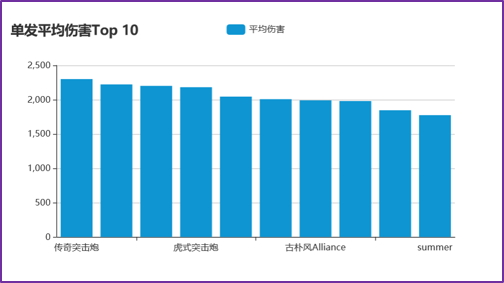
\includegraphics[width=0.45\textwidth]{statistics.png}}
    \caption{游戏数据库设计背景}
    \label{fig:chap3:resultPWF}
  \end{figure}
\subsection{数据流图}
  我们对游戏的DLL文件进行反编译(dnspy),找到了其中的坦克属性、伤害、战斗结果等消息处理函数,并让其调用外部
  我们编写的基于socket通信的DLL,在游戏过程中将数据实时发送到java进程所监听的端口。当JAVA进程接受到消息后,首先对消息类型
  做判断,接下来根据其类型进行实时GUI显示并通过JDBC存入MySQL数据库。JAVA进程还可通过查询数据库中所有的数据信息来对数据
  做统计分析展示。对于socket通信,我们采用了消息队列与生产者消费者多线程模型来保证数据的正确写入与读取。
  \begin{figure}[H] % use float package if you want it here
    \centering
    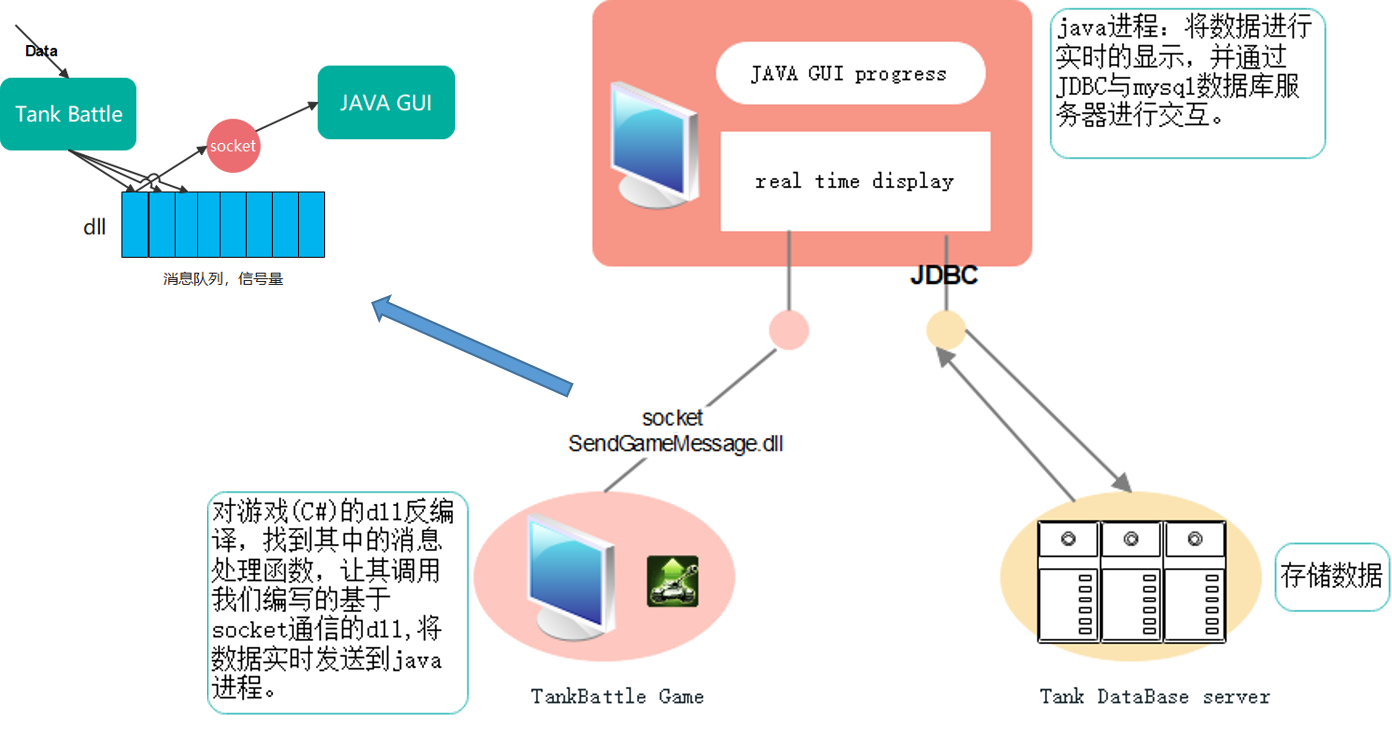
\includegraphics[width=0.95\textwidth]{dataflow.png}
    \caption{整体框架设计}
    \label{fig:chap1:structure}
  \end{figure}
\section{ER图设计说明}
\subsection{实体关系模型设计}
针对实际获取的游戏数据,我们将实体关系模型设计如图\ref{fig:erd}所示。我们总共设计了六个实体,分别是
此软件用户实体、游戏玩家实体、坦克实体、战斗数据实体、战斗结果实体、评论实体。其中软件用户实体与游戏玩家实体是
多对一的绑定关系,即多个软件用户可以绑定同一个游戏账号,便于后续的个人游戏战绩统计与分析。每次攻击伤害仅来自于一名
玩家,而每个玩家可以有若干条的伤害记录,因此玩家实体与伤害实体为一对多的关系。每次伤害都有一辆攻击坦克与被攻击坦克,因此伤害实体与坦克实体间
有两个多对一的攻击与受害的关系。游戏战斗结果与玩家实体、坦克实体是多对一的关系,即一个玩家可以使用一种坦克产生多条的
战斗结果数据。此外软件用户实体可以对某一条战斗结果或战斗伤害进行评论。
 \begin{figure}[h] % use float package if you want it here
    \centering
    \includegraphics[width=0.95\textwidth]{erd.png}
    \caption{ER图设计}
    \label{fig:erd}
  \end{figure}
\subsection{各表属性与约束设计}

1)软件用户user表,软件用户表记录了此软件的使用者的基本信息,其属性如表\ref{tab:user}所示,user\_id为主键。
\begin{table}[H]
\centering
\caption{软件使用用户user表}\label{tab:user}
\begin{tabular}{|c|c|c|c|c|c|c|c|c|}\hline
user\_id&nickname&password&mobile&email&gender&birthday&address&registartion\_time \\\hline
用户ID&用户昵称&密码&手机&邮箱&性别&生日&地址&注册时间\\\hline
\end{tabular}
\end{table}

2)用户绑定玩家表(user\_bindplayer),
该表记录了此软件用户绑定游戏账户昵称信息。其中主键为(user\_id, playerName),外键约束为user\_id参考user表,
playerName参考playerinfo表。因为软件用户与游戏玩家是一个多对一的关系,因此设计用户绑定玩家表便于数据库信息维护。
\begin{table}[H]
\centering
\caption{user\_bindplayer表}\label{tab:userbind}
\begin{tabular}{|c|c|c|}\hline
user\_id&playerName&bind\_time\\\hline
软件用户ID&绑定游戏昵称&绑定时间\\\hline
\end{tabular}
\end{table}

3)玩家表(playerInfo)
该表记录了玩家的游戏的昵称
\begin{table}[H]
\centering
\caption{user\_bindplayer表}\label{tab:userbind}
\begin{tabular}{|c|c|}\hline
playerId&playerName\\\hline
玩家ID&玩家游戏昵称\\\hline
\end{tabular}
\end{table}

4)Tank表(tank),图\ref{fig:tank}所示,该表记录了从游戏中获取的坦克信息,其中tankkind为主键(该值为游戏定义),tankName为坦克名称,tankClass为坦克类型,tankGrade为坦克等级,tankDescription为对坦克的文字描述。

 \begin{figure}[h]
    \centering
    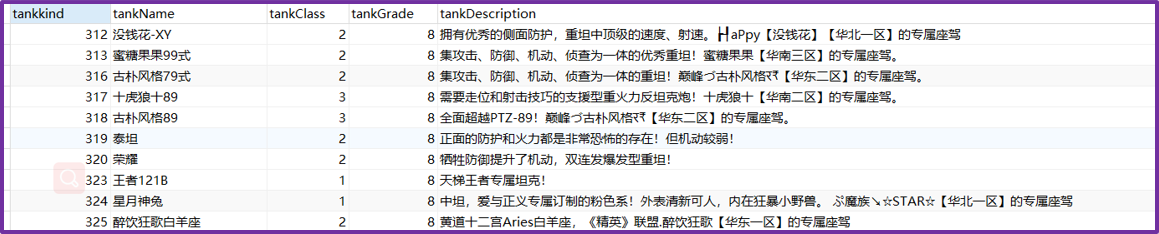
\includegraphics[width=1\textwidth]{tank.png}
    \caption{tank表与部分数据}
    \label{fig:tank}
  \end{figure}

5)战斗伤害表(battleDamage),\ref{fig:damage}该表记录了玩家使用某坦克在战场上造成的单发伤害信息。其中battle\_damage\_id为单次攻击伤害id,attackerPlayerName为攻击玩家昵称,attackerKind为攻击坦克类型,victimeKind为受害坦克类型,damage为伤害值,damageKind为伤害类型,
battleMode为此次伤害所处的游戏模式,IsFriend表示是否为友军伤害,属性battleTime为造成伤害的时间。该表的主键为battle\_damage\_id,外键attackPlayerName参考PlayerInfo表,外键attackerKind与victimKind参考tank表tankkind字段。
 \begin{figure}[h]
    \centering
    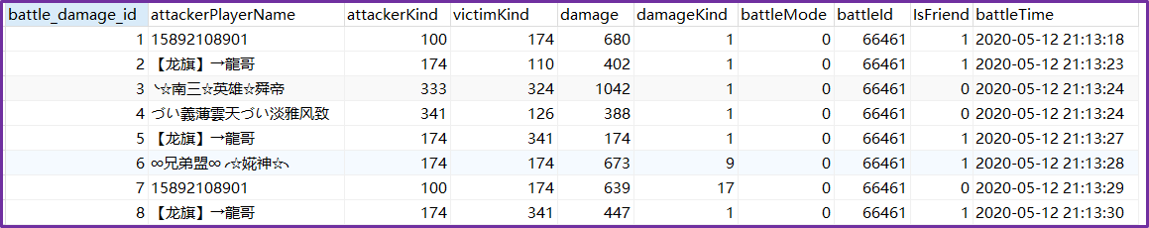
\includegraphics[width=1\textwidth]{damage.png}
    \caption{战斗伤害表与部分数据}
    \label{fig:damage}
  \end{figure}

6)战斗结果表(battleResult),该表记录了某个玩家使用坦克的战斗结果的详细数据信息。其中battleResult\_id为战斗结果id(主键),victory表示战斗是否胜利,survival为玩家坦克是否存活,enemiesdestroyed为该玩家本场摧毁的坦克数量,damagecaused为玩家本场战斗总伤害值,
damagereceived为本场战斗的承受伤害,shotsfired为开火次数,hits为命中次数,penetrations为穿透次数,battlemode表示游戏模式,属性battletime为结算时间。
该表的主键为BattleResult\_id唯一标识某位玩家某一时刻的战斗结果。外键PlayerName参考玩家表,tankKind参考tank表,使用外键可以消除玩家与坦克其他信息的冗余,且满足第三范式。
 \begin{figure}[h]
    \centering
    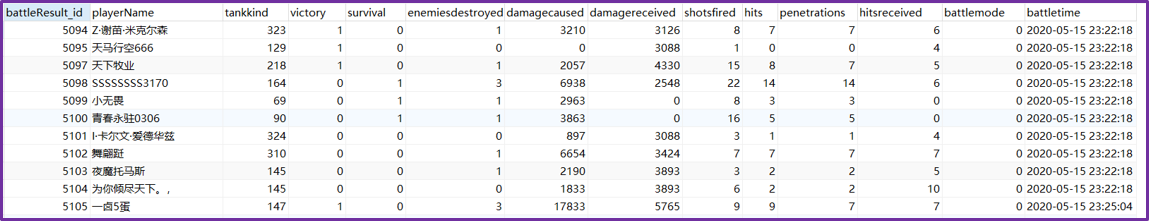
\includegraphics[width=1\textwidth]{result.png}
    \caption{战斗结果表与部分数据}
    \label{fig:damage}
  \end{figure}

7)战斗评论表(userCommentResult),该表记录了软件用户对某条战斗结果的评价。外键user\_id参考user表,BattleResult\_id参考
BattleResult表。
\begin{table}[H]
\centering
\caption{userCommentResult表}\label{tab:usercomment}
\begin{tabular}{|c|c|c|c|}\hline
user\_id&battleResult\_id&comment&comment\_time\\\hline
软件用户ID&战斗结果ID&评论内容&评论时间\\\hline
\end{tabular}
\end{table}

\section{数据库操作说明}
\subsection{基本的增删改查}
为了便于小组间协作,我们的MySQL数据库位于阿里云服务器,IP地址123.56.118.161,端口为3306。用户名为root,密码为123456。
限于篇幅的原因,基本增删改查分别举一例进行介绍。

插入语句:此软件需要用户注册后才能够使用,向数据库中添加用户信息。
\begin{lstlisting}[style=A]
INSERT INTO `user`(`nickname`,`userPassword`,`mobile`,`email`,`gender`,`birthday`,`address`) VALUES
('user2', '123456','13121265866','abletian@gmail.com','男',NULL,NULL),
('user3','123456','15548972058','123084784@qq.com','女',NULL,NULL)
\end{lstlisting}

删除语句:玩家对自己的战斗结果数据进行美化,删除自己零伤的战斗记录。
\begin{lstlisting}[style=A]
DELETE FROM `battleResult`
WHERE `playerName` = '我要空降皇后(无情)'AND `damagecaused` = 0;
\end{lstlisting}

更改语句:软件用户对用户信息进行更新
\begin{lstlisting}[style=A]
UPDATE user SET `nickname`= '这个杀手有点冷',mobile='13121265866' 
WHERE  `user_id` = 1
\end{lstlisting}

查询语句:查询某软件用户绑定的游戏玩家昵称信息。
\begin{lstlisting}[style=A]
SELECT playerName FROM `user` 
INNER JOIN user_bindplayer ON `user`.user_id = user_bindplayer.user_id
WHERE nickname = '空降皇后无情'
\end{lstlisting}

\subsection{复杂查询语句与视图}
游戏数据实时写入数据库均通过底层的API调用自动完成,截至目前,数据库已经导入近六万条数据。
数据库的复杂操作主要针对坦克数据查询以及用
户数据查询,现将主要功能列举如下:

1)使用battleDamage数据查询PVP模式下各种坦克的暴击率,并按照降序排列取前20名,其中damageKind为9表示暴击,1为普通攻击。

\begin{lstlisting}[style=A]
  SELECT `tankName`, COUNT(`damageKind` = 9 OR NULL)/ COUNT(`damageKind` IN (1, 9) OR NULL) as 'criticalrate'
  FROM `battleDamage` INNER JOIN `tank` on `battleDamage`.attackerKind = `tank`.tankkind
  WHERE `battleDamage`.battlemode = 0
  GROUP BY `battleDamage`.attackerKind
  ORDER BY `criticalrate` desc
  LIMIT 20
/*运用battleDamage数据查询PVP模式下各种坦克的暴击率*/
\end{lstlisting}

2)使用battleDamage数据查询PVP模式下各种坦克的单发平均伤害,并进行排名显示。
\begin{lstlisting}[style=A]
SET @rownum=0;						
SELECT  @rownum:=@rownum+1 as rownum, `TB`.*
FROM(
SELECT `tankName`, AVG(damage) as 'Average damage per shot'
FROM `battleDamage` INNER JOIN `tank` on `battleDamage`.attackerKind = `tank`.tankkind
WHERE `battleDamage`.battlemode = 0
GROUP BY `battleDamage`.attackerKind
ORDER BY `Average damage per shot` desc
LIMIT 20
) As `TB`
/*运用battleDamage数据查询PVP模式下各种坦克的单发平均伤害/
\end{lstlisting}

3)与上面两个查询类似,我们还实现了命中率、击穿率、单发平均伤害、 单发最高伤害、坦克胜率、存活率、 
单场伤害、场均伤害、单场承受伤害、场均承受伤害、场均被击中次数、场均击毁敌人数等全服坦克信息的查询,详情请参考
提交的查询sql文件。

4)查询某一用户所绑定玩家的全部游戏记录。在该查询中我们创建了用户比赛信息视图userbattleinfo,便于查询。
\begin{lstlisting}[style=A]
  CREATE VIEW userbattleinfo AS
  SELECT
	`battleResult`.`playerName` AS `playerName`,
	`user_bindplayer`.`user_id` AS `user_id`,
	`tank`.`tankName` AS `tankName`,
	`battleResult`.`tankkind` AS `tankKind`,
	`battleResult`.`victory` AS `victory`,
	`battleResult`.`survival` AS `survival`,
	`battleResult`.`enemiesdestroyed` AS `enemiesdestroyed`,
	`battleResult`.`damagecaused` AS `damagecaused`,
	`battleResult`.`damagereceived` AS `damagereceived`,
	`battleResult`.`shotsfired` AS `shotsfired`,
	`battleResult`.`hits` AS `hits`,
	`battleResult`.`penetrations` AS `penetrations`,
	`battleResult`.`hitsreceived` AS `hitsreceived`,
	`battleResult`.`battlemode` AS `battlemode`,
	`battleResult`.`battletime` AS `battletime`
FROM
	(
		(
			`battleResult`
			JOIN `user_bindplayer` ON (
				(
					`battleResult`.`playerName` = `user_bindplayer`.`playerName`
				)
			)
		)
		JOIN `tank` ON (
			(
				`battleResult`.`tankkind` = `tank`.`tankkind`
			)
		)
	)
ORDER BY
	`battleResult`.`battletime` DESC
/*创建用户比赛信息视图userbattleinfo,便于查询/
\end{lstlisting}

\begin{lstlisting}[style=A]
  SELECT *
  FROM `userbattleinfo`
  where user_id=7
/*查询某一用户的全部游戏记录/
\end{lstlisting}

5)查询用户绑定的玩家使用不同坦克的战斗情况,包含每辆坦克的出战次数、胜率、存活率、场均伤害、
场均承受伤害、场均被命中次数、场均击毁数、场均命中率、场均穿透率,并按照出战次数降序排列。
图\ref{fig:userresult}为某一玩家的查询显示结果。
\begin{lstlisting}[style=A]
SELECT tankName, COUNT(tankkind) as `usingtimes`, 
COUNT(`victory`=0 or Null)/COUNT(tankkind) as 'win rate',
COUNT(`survival`=1 or Null)/COUNT(tankkind) as 'survival rate', 
AVG(`damagecaused`) as 'average damage casued',
AVG(`damagereceived`) as 'average damage received', 
AVG(`hitsreceived`) as 'average hits received',
AVG(`enemiesdestroyed`) as 'average enemies destroyed',
SUM(`hits`)/SUM(`shotsfired`) as 'accuracy',
SUM(`penetrations`)/SUM(`shotsfired`) as 'penetration rate'
FROM `userbattleinfo`
WHERE `user_id`=7
GROUP BY `tankkind`
ORDER BY `usingtimes` desc;	
/*查询某一用户的坦克情况/
\end{lstlisting}
 \begin{figure}[h]
    \centering
    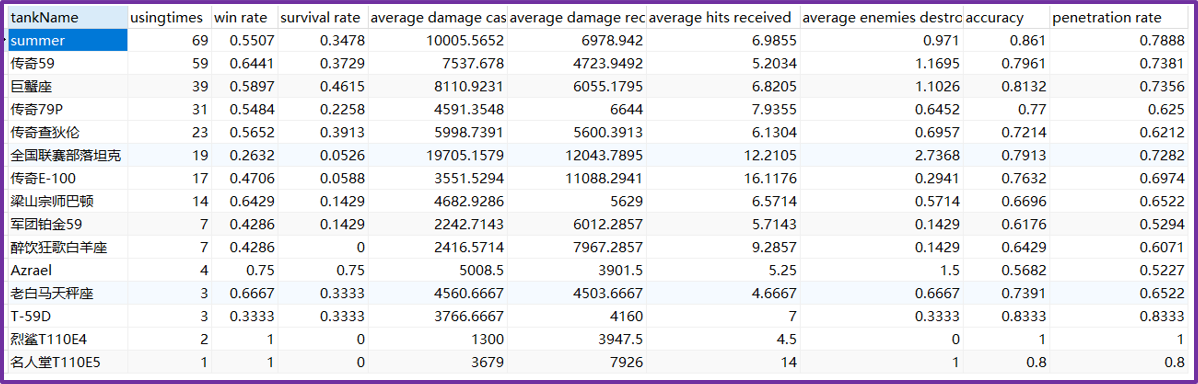
\includegraphics[width=1\textwidth]{userresult.png}
    \caption{某玩家使用不同坦克的出战情况}
    \label{fig:userresult}
  \end{figure}

\section{可视化界面说明}

图\ref{fig:code}所示为JAVA GUI界面的代码文件树状图。lib目录为java所需要的的外部库,如JDBC等。
resource文件夹为GUI界面所需要使用的图片。src文件夹为界面的java源码。

对于接收到的游戏数据总共设计了三个类,BattleResult.java、Damage.java、TankInfo.java分别对应坦克基本信息,
战斗中的单发伤害信息,战斗结果信息,这三个类将接收到的字符串转化为相应的java对象。MysqlAPI.java完成数据库服务器的连接,
并提供将得到的游戏数据写入到数据库的函数接口。DrawDamage.java对接收到的实时伤害数据做一个动态的显示。ServerProxy.java
对本地端口进行监听,当接收到游戏进程发送过来的数据后,做进一步的处理。TankBox.java为基本的登录注册界面。TankBoxUserPanel.java
为用户登录后的功能界面,如查看今日战绩、实时伤害数据、全服坦克大数据。
\subsection{代码简单说明}

ServerProxy.java是一切数据处理的起点,部分核心代码如下,改段代码为当有端口有数据写入后,首先根据数据类型做分类,
然后发送到不同的case中去执行,有的直接存入数据库,有的则还进行实时显示。
\begin{lstlisting}[style=A]
  while((temp = bw.readLine())!= null)
            {
                try{
                    if(temp != null){
                        String[] result = temp.split(",", 2);
                        switch (result[0]){
                            case "3":
                                BattleResult br = new BattleResult(temp);
                                if(br.mKind != -1) {
                                    MysqlAPI.addBattleResult(br);
                                }
                                break;
                            case "1":
                            case "5":
                                TankBoxUserPanel.drawDamage.PushString(temp);
                                TankBoxUserPanel.drawDamage.repaint();
                                TankBoxUserPanel.drawDamage.updateUI();
                                Damage damage = new Damage(temp);
                                if(damage.mAttackerKind != -1){
                                    MysqlAPI.addBattleDamage(damage);
                                }
                                break;
                            case "6":
                                TankInfo tankinfo = new TankInfo(temp);
                                if(tankKinds.contains(Integer.valueOf(tankinfo.tankKind))){
                                    break;
                                }else{
                                    MysqlAPI.addTankInfo(tankinfo);
                                }
                            default:
                                break;
                        }
                    }
\end{lstlisting}

\subsection{操作步骤和功能}
1)注册登录
  \begin{figure}[h]
    \centering
    \subcaptionbox{注册界面\label{fig:subfig11}}
        {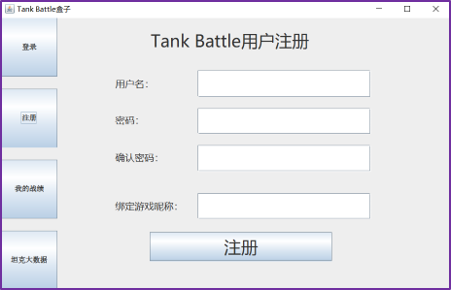
\includegraphics[width=0.45\textwidth]{regis.png}}
    \hspace{0.05\textwidth}
    \subcaptionbox{登录界面\label{fig:subfig22}}
        {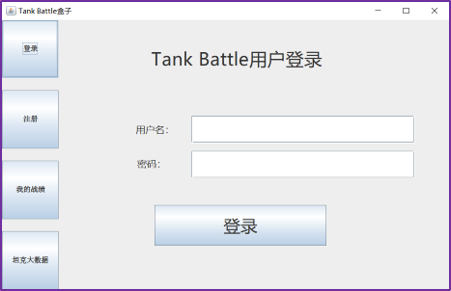
\includegraphics[width=0.45\textwidth]{login.png}}
    \caption{软件注册登录界面}
    \label{fig:chap3:logreg}
  \end{figure}

2)实时伤害显示,绿色为友军坦克名称,红色为敌军,后面为伤害与伤害类型。
  \begin{figure}[h]
    \centering
    \subcaptionbox{实时伤害数据\label{fig:subfig11}}
        {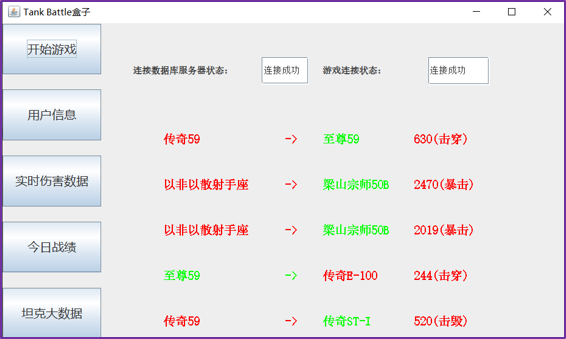
\includegraphics[width=0.45\textwidth]{realtimeDamage.png}}
    \hspace{0.05\textwidth}
    \subcaptionbox{我的今日战绩\label{fig:subfig22}}
        {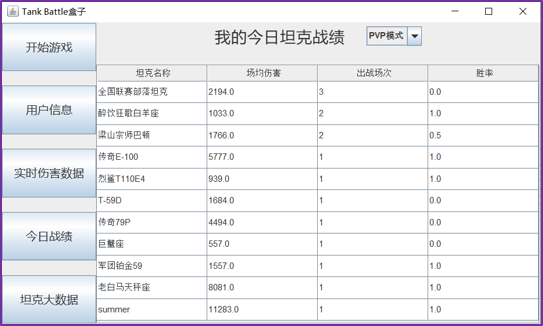
\includegraphics[width=0.45\textwidth]{todayresult.png}}
    \caption{用户登录后界面}
    \label{fig:chap3:logreg}
  \end{figure}

3)我的今日战绩,基于坦克战斗结果表与当前用户绑定玩家信息,对该玩家本日的战斗数据做统计分析,包含不同坦克场均伤害、出战场次、胜率信息。


4)全服坦克大数据,基于伤害表与战斗结果表,我们统计了全服坦克大数据信息包含暴击率、命中率、击穿率、单发平均伤害、 单发最高伤害、坦克胜率、存活率、 单场伤害、场均伤害、单场承受伤害、场均承受伤害、场均被击中次数、场均击毁敌人数等。
 \begin{figure}[h]
    \centering
    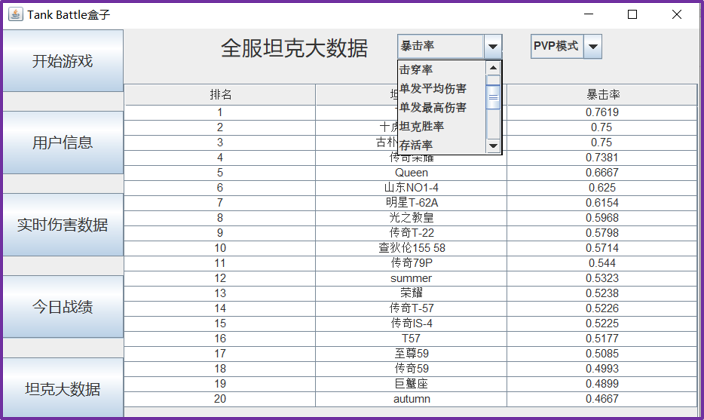
\includegraphics[width=0.7\textwidth]{total.png}
    \caption{全服坦克大数据}
    \label{fig:total}
  \end{figure}


\section{提交文件说明}

TankStream文件夹为JAVA可视化界面代码

GameStart文件夹为基于Windows API的游戏启动exe代码,避免游戏官方启动器的DLL文件效验。

DLL\_SendMessage文件夹为编写的基于socket通信的DLL

大作业报告文件夹包含了报告与报告的tex源文件

TankBattle.pptx为展示PPT

CreateTable.sql与Select.sql为建表与查询的SQL语句

坦克大战源码分析.md为对游戏源码反编译后修改的记录

整个项目的github地址:\url{https://github.com/sty16/Tank-Battle-Box}
 \begin{figure}[h]
    \centering
    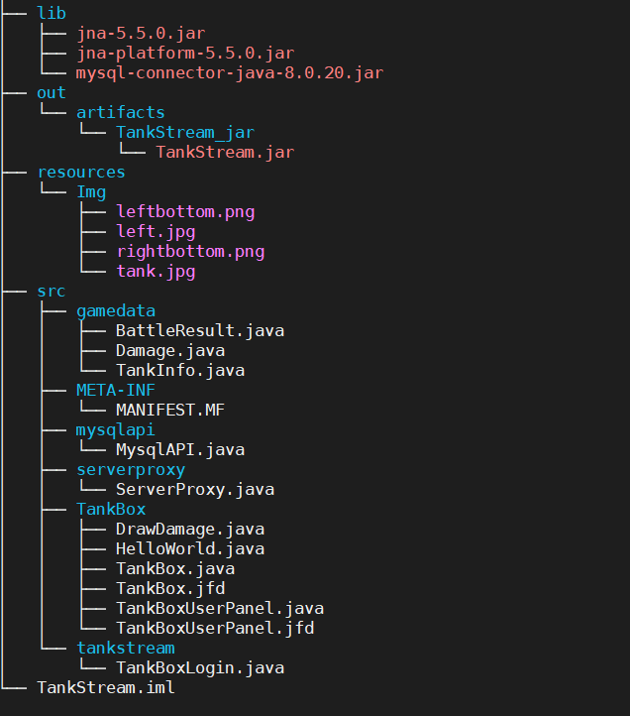
\includegraphics[width=1\textwidth]{code.png}
    \caption{java可视化界面文件说明}
    \label{fig:code}
  \end{figure}
\end{document}
